%%% Template originaly created by Karol Kozioł (mail@karol-koziol.net) and
%%% modified for ShareLaTeX use

\documentclass[a4paper,12pt]{report}

\usepackage[
  backend=biber,
  style=authoryear-ibid, % Motsvarar agsm.
  uniquename=init,
  giveninits,  % Ersätt hela förnamn med bara initialerna.
  maxnames=2,  % Ersätt med et al./m.fl. om det är fler än två förf.
  natbib=true,
  hyperref=true,
  backref=true,
  doi=false,
  isbn=false,
  url=false
]{biblatex}
\addbibresource{exjobb.bib}
% Lite kortare referenslista utan URL:er och DOI:er.

\usepackage{csquotes} % Must be before babel.
\usepackage[american]{babel}
\usepackage[T1]{fontenc}
\usepackage[utf8]{inputenc}
\usepackage{pdfsync}
\synctex=1
\usepackage{parskip} % Package to tweak paragraph skipping.
\usepackage{hyperref}
\usepackage{xcolor}

\usepackage{fancyhdr}

\renewcommand\familydefault{\sfdefault}
\usepackage{tgheros}
\usepackage[defaultmono]{droidmono}
\usepackage[framed,numbered]{matlab-prettifier}
\makeatletter
\newcommand\BeraMonottfamily{%
  \def\fvm@Scale{0.6}% scales the font down
  \fontfamily{fvm}\selectfont% selects the Bera Mono font
}
\makeatother

\usepackage{amsmath,amssymb,amsthm,textcomp}
\usepackage{enumerate}
\usepackage{multicol}
\usepackage{tikz}
\usepackage{caption,subcaption}

\usepackage{calc}
\newenvironment{altDescription}[1][\quad]
  {\begin{list}{}{
   \renewcommand\makelabel[1]{\hfil\textsf{##1}}
   \settowidth\labelwidth{\makelabel{#1}}
   \setlength\leftmargin{\labelwidth+\labelsep}}}
  {\end{list}}

\title{Bachelor's thesis}
\author{Jonas Nockert, nockert@kth.se}
\date{2018}

\begin{document}

\maketitle

\section{Bakgrund}


* Förvånansvärt lite teori bakom skotträning och var man ska skjuta (cf.
Magnusson).





För att bli en bra målskytt inom ishockey behöver en spelare skjuta åtminstone
100--200 skott om dagen. Tiden på isträningen räcker inte till för detta och
på senare år har därför Svenska Ishockeyförbundet börjat uppmuntra spelare
att träna med skottramp (\citep{Swehockey:2016}). Det är numera vanligt att
klubbar och spelare (på alla nivåer) bygger skottramper och använder dem
för daglig träning.

\begin{figure}[ht]
  \centering
  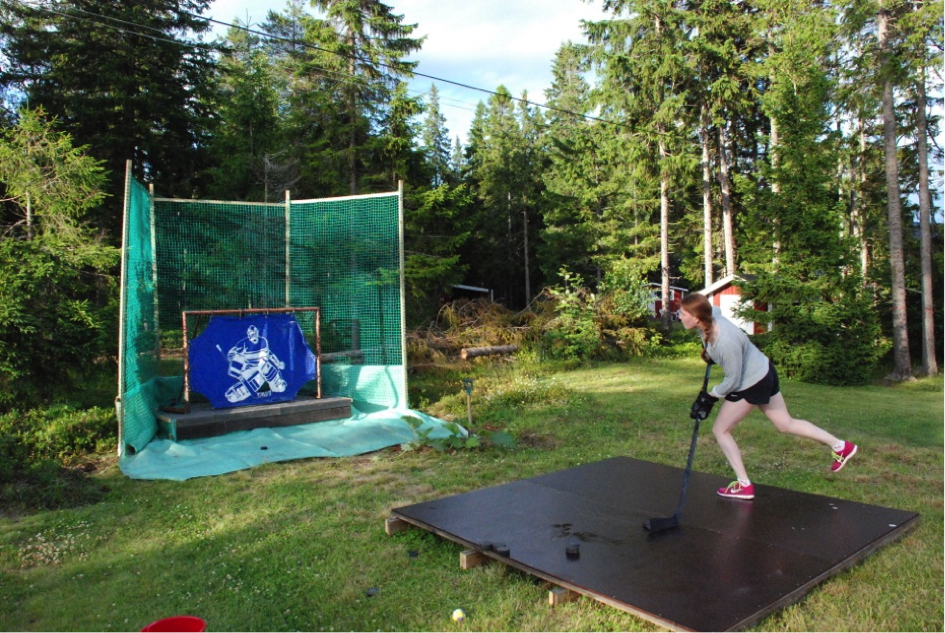
\includegraphics[width=\linewidth]{photos/the-incredible-shooting-ramp-my-mom-built-for-me.png}
  \caption{Exempel på skottrampsträning utomhus
  (\href{https://yalewomenshockey.wordpress.com/2013/07/18/ywih-summer-blog-hanna-astrom/}{YALE Womens Hockey's Blog}).
  \label{fig:skottramp}}
\end{figure}

Målvakterna blir allt skickligare så det gäller att träna på ett sätt
så chanserna att göra mål eller i alla fall bidra till att göra mål blir så
stora som möjligt. Det gäller att lära sig skjuta hårda skott med precision
men också att minska tiden mellan att få pucken och att skjuta. Det dröjer
inte länge innan målvakten har hunnit positionera sig på ett sätt att
luckorna att göra mål blivit väldigt små.

En vanlig metod vid skottrampsträning är att använda en duk med öppningar
motsvarande de luckor en målvakt oftare än andra lämnar öppna (se
figur~\ref{fig:duk}).

\begin{figure}[ht]
  \centering
  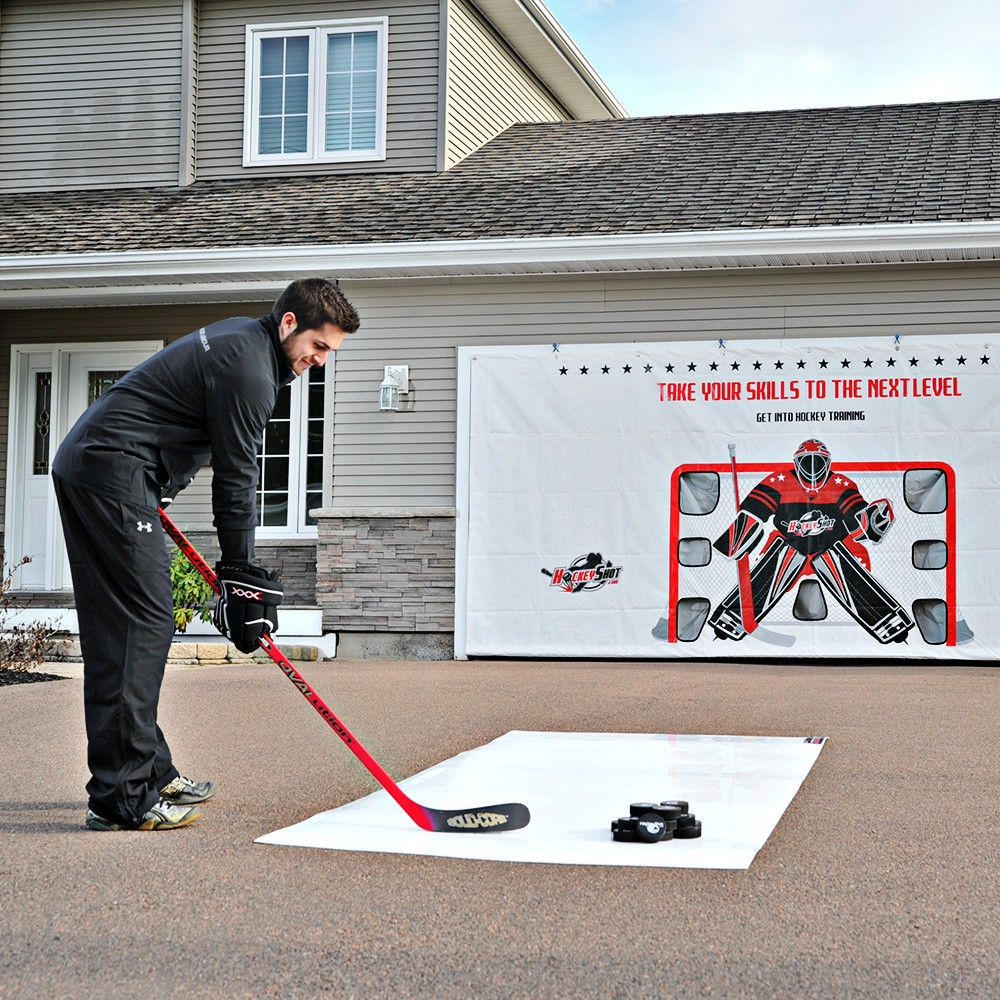
\includegraphics[width=\linewidth]{photos/shooting-tarp.jpg}
  \caption{Exempel på duk
  (\href{http://www.hockeyshot.se/HockeyShot-Extreme-Shooting-Tarp-p/target-tarp-032.htm}{hockeyshot.se}).
  \label{fig:duk}}
\end{figure}

En spelare som blandar olika skottyper och skjuter 100--200 skott om dagen
blir förstås bättre över tid men det är en långsam process och det kan vara
svårt att hålla uppe motivationen. En fördel vore om det gick att
kontinuerligt kvantifiera resultat och förbättringar och på så sätt kunna
hjälpa till med motivation samt långsiktig systematisering av träningen.

Idrottsforskaren Johnny Nilsson har tillsammans med kollegor på Dalarna
University filmat skottrampsträningar och manuellt analyserat resultatet
för att få fram statistisk information vad gäller träffbild och resultat
över tid. Problemet är att detta är mycket tidskrävande och ger en stor
fördröjning av återkopplingen till spelaren. Att uppnå god precision på
centimeternivå är betydligt svårare än vad det verkar vid en första anblick,
något som kan ses i figur~\ref{fig:skott}.

\begin{figure}[ht]
  \centering
  \begin{subfigure}[t]{0.24\textwidth}
    \centering
    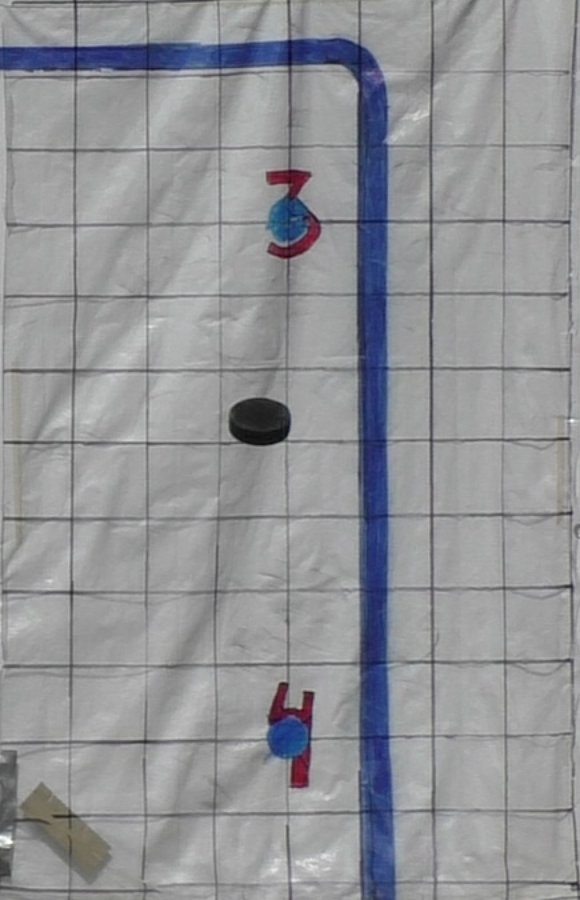
\includegraphics[width=\linewidth]{photos/skott1.png}
  \end{subfigure}%
  \hspace*{\fill}
  \begin{subfigure}[t]{0.24\textwidth}
    \centering
    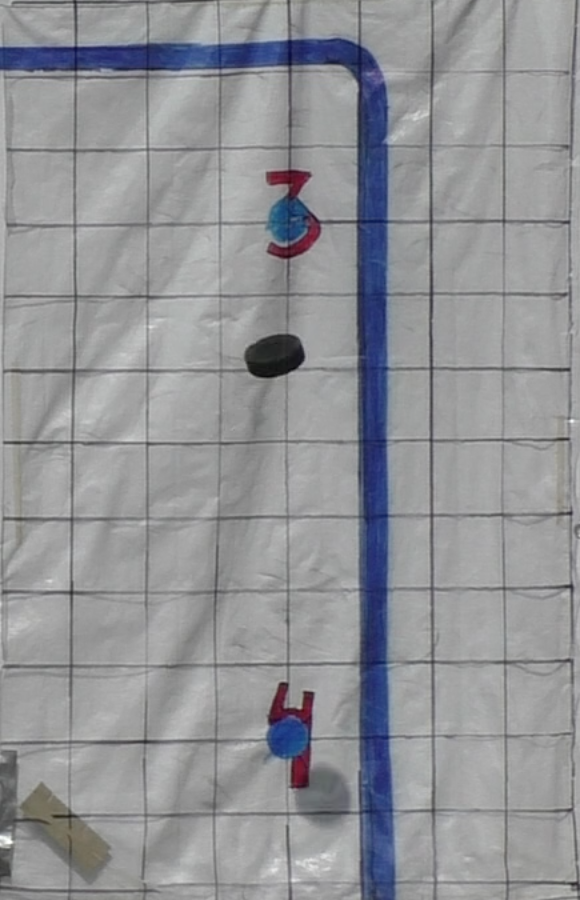
\includegraphics[width=\linewidth]{photos/skott2.png}
  \end{subfigure}%
  \hspace*{\fill}
  \begin{subfigure}[t]{0.24\textwidth}
    \centering
    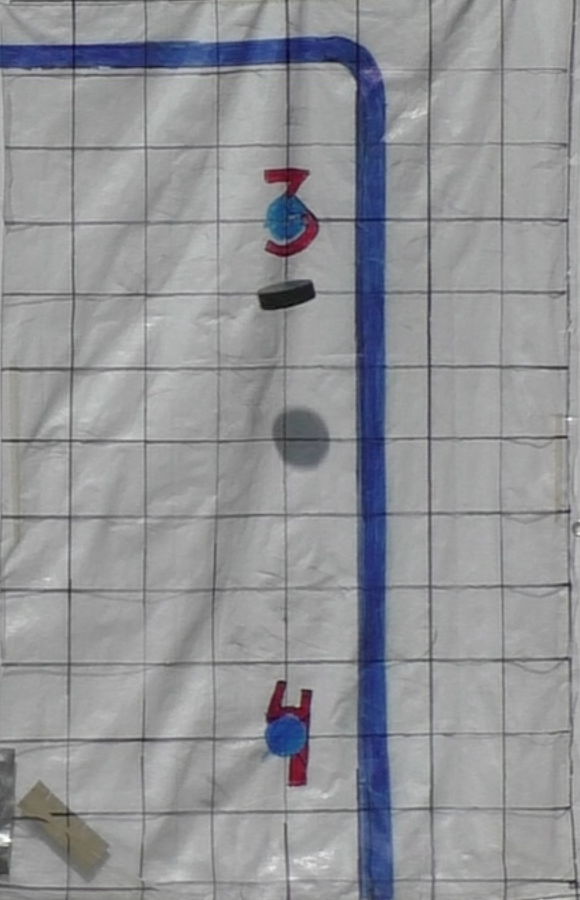
\includegraphics[width=\linewidth]{photos/skott3.png}
  \end{subfigure}%
  \hspace*{\fill}
  \begin{subfigure}[t]{0.24\textwidth}
    \centering
    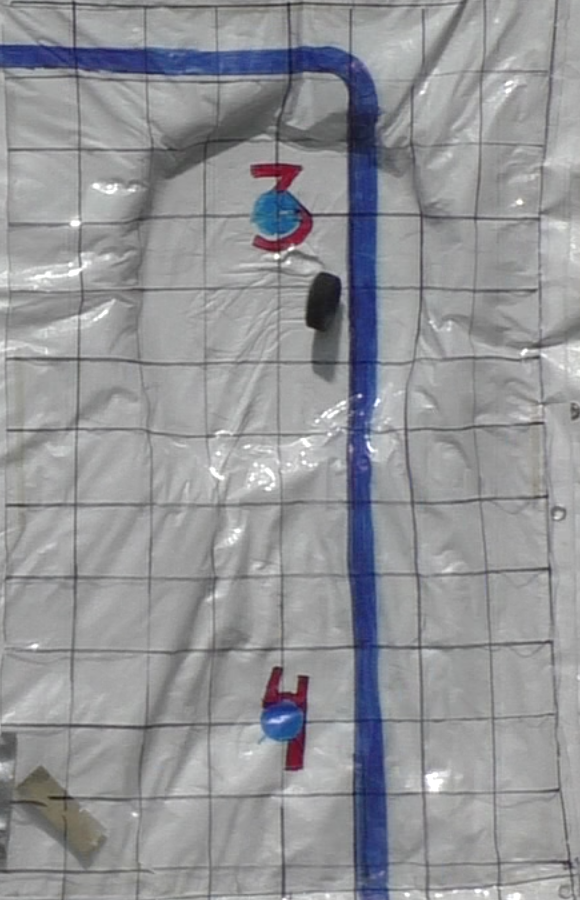
\includegraphics[width=\linewidth]{photos/skott4.png}
  \end{subfigure}%

  \caption{Även manuellt kan det vara svårt att avgöra exakt var pucken
    träffar. Utsnitt ur träningsserie, filmad med videokamera och 60 fps.}
  \label{fig:skott}
\end{figure}

% Under våren 2017 formerades ett MVK-projekt runt problemet och en applikation
% togs fram där träningsfilmer spelades in med hjälp av mobiltelefon som sedan
% skickades till en server i molnet för analys. Det tog lång tid att analysera
% och på så sätt fördröjdes återkopplingen till långt efter träningen tagit
% slut.

Eftersom det bara tar en sekund att få iväg ett hockeyskott så finns det
endast ett kort fönster att påbörja återkoppling innan spelaren skjuter nästa
skott. Efter det får en sammanfattad återkoppling istället ske efter
träningen.

En automatisering på ett liknande sätt som det Nilsson etablerat
kräver både mycket processorkraft och hög grad av integration mellan
inspelning och bildanalys, något som t.ex. moderna mobiltelefoner erbjuder.

%% \citet[]{McMillan:2012}

\subsection{(a)}\label{sec:part1a}

\begin{figure}
  \begin{tikzpicture}[
    % scale=0.5,
    % level/.style={thick}
    ]
    \draw (-2.5,-2) node[anchor=north]{Precise}
       -- (0,2) node[anchor=south]{Hard}
       -- (2.5,-2) node[anchor=north]{Fast}
       -- cycle;
     \circle
  \end{tikzpicture}
\end{figure}





För att etablera en bakgrundsmodell behövs ett antal sekunder av enbart
"bakgrund", det kan applikationen göra genom att fördröja tiden innan första
skottet (något som ändå måste göras ifall spelaren själv ska starta appen).




%%
%% Appendix
%%

\pagebreak
\section{Appendix: Matlabkod}

\printbibliography{}
\end{document}
